\chapter{Agile, Scrum, CI/CD \& DevOps}
\label{ch:agile}

The final chapter turns to modern delivery: agile values, Scrum mechanics, and the CI/CD and DevOps practices that enable continuous delivery at scale. These ideas are not opposed to earlier chapters---they complement rigorous requirements, modelling, and testing with faster feedback.

\section{Agile Manifesto and Principles}

Agile (2001) values \emph{individuals and interactions} over processes and tools, \emph{working software} over comprehensive documentation, \emph{customer collaboration} over contract negotiation, and \emph{responding to change} over following a plan. Twelve principles elaborate: satisfy the customer through early continuous delivery, welcome changing requirements, deliver frequently (weeks not months), daily collaboration between business and developers, sustainable pace, and continuous attention to technical excellence.

Agile is not ``no process'' or ``no documentation.'' It is \emph{just enough} process and documentation, continuously refined.

\section{Scrum Framework}

Scrum is the most widely adopted agile framework, with three roles, three artefacts, and five events.

\begin{itemize}
    \item \textbf{Roles}: Product Owner (owns and prioritises the backlog, maximises value), Scrum Master (facilitates process, removes impediments), Development Team (cross-functional, self-organising, $3$--$9$ members).
    \item \textbf{Artefacts}: Product Backlog (ordered list of all desired work), Sprint Backlog (selected items for the current sprint plus plan), Increment (potentially shippable working software).
    \item \textbf{Events}: Sprint ($1$--$4$~weeks, time-boxed), Sprint Planning, Daily Scrum ($15$~min stand-up), Sprint Review (demo to stakeholders), Sprint Retrospective (process improvement).
\end{itemize}

\begin{figure}[h]
\centering
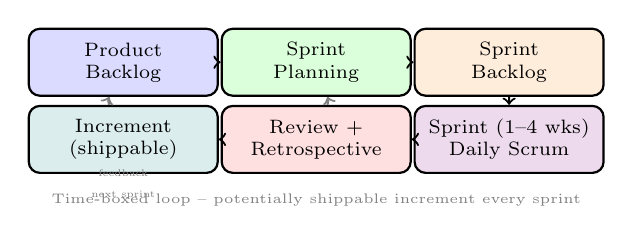
\begin{tikzpicture}[scale=0.70, every node/.style={font=\scriptsize}]
  \tikzstyle{box}=[draw,rounded corners,minimum width=2.4cm,minimum height=0.85cm,align=center,thick]
  \node[box,fill=blue!14] (pb) at (0,2.2) {Product\\Backlog};
  \node[box,fill=green!14] (plan) at (3.5,2.2) {Sprint\\Planning};
  \node[box,fill=orange!14] (sb) at (7.0,2.2) {Sprint\\Backlog};
  \node[box,fill=violet!14] (sprint) at (7.0,0.8) {Sprint (1--4 wks)\\Daily Scrum};
  \node[box,fill=red!12] (rev) at (3.5,0.8) {Review +\\Retrospective};
  \node[box,fill=teal!14] (inc) at (0,0.8) {Increment\\(shippable)};
  \draw[->,thick] (pb) -- (plan);
  \draw[->,thick] (plan) -- (sb);
  \draw[->,thick] (sb) -- (sprint);
  \draw[->,thick] (sprint) -- (rev);
  \draw[->,thick] (rev) -- (inc);
  \draw[->,thick,dashed,gray,bend left=22] (inc) to (pb) node[midway,above,font=\tiny] {feedback};
  \draw[->,thick,dashed,gray,bend right=18] (rev) to (plan) node[midway,below,font=\tiny] {next sprint};
  \node[font=\tiny,gray,align=center] at (3.5,-0.3) {Time-boxed loop -- potentially shippable increment every sprint};
\end{tikzpicture}
\caption{Scrum flow -- ordered backlog feeds sprint planning; each sprint delivers a shippable increment; review and retrospective close the loop.}
\end{figure}

\begin{figure}[h]
\centering
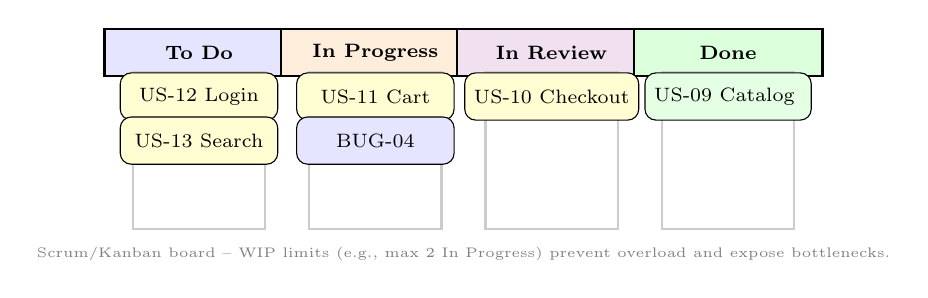
\begin{tikzpicture}[scale=0.70, every node/.style={font=\scriptsize}]
  % Scrum board columns
  \foreach \x/\lbl/\col in {0/To Do/blue!10, 3.2/In Progress/orange!14, 6.4/In Review/violet!12, 9.6/Done/green!14} {
    \node[draw,fill=\col,minimum width=2.4cm,minimum height=0.6cm,align=center,thick] at (\x,1.8) {\textbf{\lbl}};
    \draw[thick,gray!40] (\x-1.2,-1.4) rectangle (\x+1.2,1.45);
  }
  % cards
  \node[draw,fill=yellow!18,rounded corners,minimum width=2.0cm,minimum height=0.6cm,align=center] at (0,1.0) {US-12 Login};
  \node[draw,fill=yellow!18,rounded corners,minimum width=2.0cm,minimum height=0.6cm,align=center] at (0,0.2) {US-13 Search};
  \node[draw,fill=yellow!18,rounded corners,minimum width=2.0cm,minimum height=0.6cm,align=center] at (3.2,1.0) {US-11 Cart};
  \node[draw,fill=blue!10,rounded corners,minimum width=2.0cm,minimum height=0.6cm,align=center] at (3.2,0.2) {BUG-04};
  \node[draw,fill=yellow!18,rounded corners,minimum width=2.0cm,minimum height=0.6cm,align=center] at (6.4,1.0) {US-10 Checkout};
  \node[draw,fill=green!10,rounded corners,minimum width=2.0cm,minimum height=0.6cm,align=center] at (9.6,1.0) {US-09 Catalog \checkmark};
  \node[font=\tiny,gray] at (4.8,-1.85) {Scrum/Kanban board -- WIP limits (e.g., max 2 In Progress) prevent overload and expose bottlenecks.};
\end{tikzpicture}
\caption{Scrum board (task board) -- work flows left to right; work-in-progress limits keep flow smooth and make blockages visible.}
\end{figure}

Estimation uses story points (relative effort, often Fibonacci: 1, 2, 3, 5, 8, 13) rather than hours, and velocity (points per sprint) for planning. Burndown charts track remaining work within a sprint; burnup charts track scope plus progress across releases.

\section{Kanban and Lean}

Kanban visualises workflow on a board with explicit WIP limits per column (e.g., ``In Progress $\leq 3$''). Unlike Scrum's fixed sprints, Kanban is continuous flow: pull work when capacity allows, optimise for lead time and throughput. Lean software development (Poppendieck) adds principles: eliminate waste, amplify learning, decide as late as possible, deliver as fast as possible, empower the team, build integrity in, and see the whole.

\section{CI/CD Pipelines}

\begin{definition}[CI/CD]
\emph{Continuous Integration}: every push triggers automated build and test. \emph{Continuous Delivery}: every green build is deployable to production at the push of a button. \emph{Continuous Deployment}: every green build is deployed automatically.
\end{definition}

\begin{figure}[h]
\centering
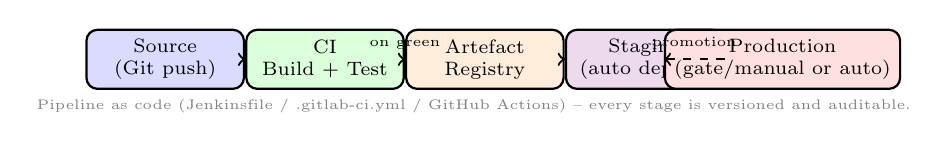
\begin{tikzpicture}[scale=0.70, every node/.style={font=\scriptsize}]
  \tikzstyle{stage}=[draw,rounded corners,minimum width=2.0cm,minimum height=0.75cm,align=center,thick]
  \node[stage,fill=blue!14] (src) at (0,0) {Source\\(Git push)};
  \node[stage,fill=green!14] (ci) at (2.9,0) {CI\\Build + Test};
  \node[stage,fill=orange!14] (art) at (5.8,0) {Artefact\\Registry};
  \node[stage,fill=violet!14] (stg) at (8.7,0) {Staging\\(auto deploy)};
  \node[stage,fill=red!12] (prod) at (11.2,0) {Production\\(gate/manual or auto)};
  \draw[->,thick] (src) -- (ci);
  \draw[->,thick] (ci) -- (art) node[midway,above,font=\tiny] {on green};
  \draw[->,thick] (art) -- (stg);
  \draw[->,thick,dashed] (stg) -- (prod) node[midway,above,font=\tiny] {promotion};
  \node[font=\tiny,gray,align=center] at (5.6,-0.85) {Pipeline as code (Jenkinsfile / .gitlab-ci.yml / GitHub Actions) -- every stage is versioned and auditable.};
\end{tikzpicture}
\caption{CI/CD pipeline -- code flows from push through automated stages to production; delivery may require manual approval, deployment does not.}
\end{figure}

Pipeline-as-code (Jenkinsfile, \texttt{.github/workflows/*.yml}) versions the pipeline alongside the product. Deployment strategies include rolling updates, blue-green (two identical environments, switch traffic), and canary (gradual traffic shift with automated rollback on error metrics).

\begin{lstlisting}[language=Python,caption={GitHub Actions CI/CD (simplified).}]
# .github/workflows/ci.yml
name: CI
on: [push, pull_request]
jobs:
  build:
    runs-on: ubuntu-latest
    steps:
      - uses: actions/checkout@v4
      - uses: actions/setup-python@v5
        with: {python-version: '3.11'}
      - run: pip install -r requirements.txt
      - run: ruff check . && pytest --cov=mypackage
      - run: docker build -t myapp:${{ github.sha }} .
\end{lstlisting}

\section{DevOps and Collaboration Culture}

DevOps unifies Development and Operations: you build it, you run it. Practices include infrastructure as code (Terraform, Ansible), observability (logs, metrics, traces), and blameless post-mortems. The CALMS model summarises: Culture, Automation, Lean, Measurement, Sharing. High-performing DevOps teams (per DORA metrics) deploy many times per day with low change-failure rates and fast recovery, because small, frequent, automated releases are safer than rare, big-bang releases.


\section{Scaling Agile and Hybrid Models}

Single-team Scrum does not automatically scale to 50~developers. Scaling frameworks include SAFe (Agile Release Trains, PI planning), LeSS (minimal extension of Scrum to multiple teams sharing one backlog), and Nexus (Scrum-of-Scrums with an integration team). All emphasise that scaling is primarily an organisational and architectural challenge, not just a process one: without a modular architecture that enables team independence, more teams create more integration pain regardless of framework.

Hybrid models are common in regulated domains: plan-driven (waterfall-style) at the system level for compliance and safety cases, agile within subsystems for faster iteration. The key is to be explicit about which practices are plan-driven and which are agile, and why.

\begin{lstlisting}[language=Python,caption={Feature flag for trunk-based development.}]
# flags.py
FLAGS = {"new_checkout": False}  # toggle without redeploy

def checkout(cart):
    if FLAGS["new_checkout"]:
        return new_checkout_flow(cart)  # incomplete work hidden
    return legacy_checkout(cart)

# Enable gradually: 1% -> 10% -> 100% with monitoring
\end{lstlisting}


\section{Metrics that Matter -- DORA and Flow}

DORA identifies four key metrics for delivery performance: deployment frequency, lead time for changes, change failure rate, and mean time to recovery (MTTR). Elite performers deploy on demand, with lead times under an hour and recovery under an hour, because small batch sizes and automation reduce both failure rate and blast radius. Flow metrics (throughput, WIP, cycle time) complement DORA by making bottlenecks visible on the board.

\begin{remark}
Adopting Scrum without engineering practices (CI, TDD, refactoring) yields ``agile in name only'': sprints produce demo-ware that cannot be shipped. Technical excellence and process agility must advance together.
\end{remark}

\section{Retrospectives and Continuous Improvement}

The retrospective is the engine of improvement: what went well, what did not, one experiment to try next sprint. Effective retrospectives are blameless, data-informed (use metrics, not anecdotes), and produce at most two action items with clear owners. Without this feedback loop, process stagnates regardless of framework.

\section{Putting It Together}

A mature team might run Scrum sprints for planning, trunk-based development with feature flags for coding, CI on every push, continuous delivery to staging, and canary deployment to production with automated rollback---all while modelling critical flows in UML and guarding quality with a testing pyramid. Process is not one choice but a coherent combination.


\section{Contract and Requirements in Agile}

Agile does not eliminate requirements; it reframes them. Fixed-price, fixed-scope contracts conflict with ``welcome changing requirements.'' Agile contracts fix time and cost but allow scope to vary within a prioritised backlog, or use incremental funding (fund one increment at a time, continue if value is demonstrated). Requirements become a continuously refined backlog rather than a frozen SRS, but traceability and acceptance criteria remain essential.


\section{Choosing Between Agile and Plan-Driven}

No single approach fits all contexts. Use plan-driven (waterfall/V-model) when requirements are stable, compliance demands traceability, and failure cost is high. Use agile when requirements are volatile, fast feedback is valuable, and the architecture allows incremental delivery. Many organisations run a hybrid: plan-driven at the portfolio level, agile within teams. The decision should be explicit and revisited as context evolves.

\begin{remark}
The most important agile practice is the retrospective. Without it, teams repeat the same mistakes every sprint and agile becomes mere ceremony.
\end{remark}

\begin{figure}[h]
\centering
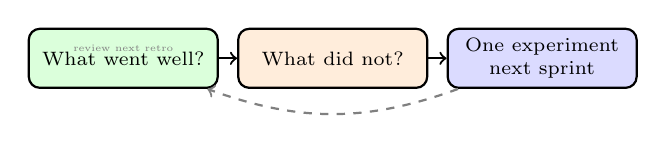
\begin{tikzpicture}[scale=0.70, every node/.style={font=\scriptsize}]
  \tikzstyle{q}=[draw,rounded corners,minimum width=2.4cm,minimum height=0.75cm,align=center,thick]
  \node[q,fill=green!14] (a) at (0,0) {What went well?};
  \node[q,fill=orange!14] (b) at (3.8,0) {What did not?};
  \node[q,fill=blue!14] (c) at (7.6,0) {One experiment\\next sprint};
  \draw[->,thick] (a) -- (b); \draw[->,thick] (b) -- (c);
  \draw[->,thick,dashed,gray,bend left=20] (c) to (a) node[midway,above,font=\tiny] {review next retro};
\end{tikzpicture}
\caption{Retrospective structure -- focus on one actionable experiment, not a laundry list that is never followed up.}
\end{figure}

\begin{remark}
DevOps is a culture before it is a toolchain. Buying a CI server without changing how dev and ops collaborate yields automation without improvement.
\end{remark}

\section{Exercises}

\begin{exercise}
Contrast Scrum roles (Product Owner, Scrum Master, Development Team) with traditional project roles (Project Manager, Analyst, Tester). Who is accountable for maximising product value, and why is the Scrum Master not a manager?
\end{exercise}

\begin{exercise}
A team completes 28, 32, 30 story points in three sprints. They have 60~points remaining and a 2-sprint deadline. Using velocity, assess feasibility and propose two concrete scope or process adjustments.
\end{exercise}

\begin{exercise}
Explain the difference between continuous delivery and continuous deployment. When would you choose delivery (manual gate) over deployment (fully automatic)? Give a domain example for each.
\end{exercise}

\begin{exercise}
Design a CI/CD pipeline for a Python microservice: list stages, triggers, quality gates, and deployment strategy (blue-green vs.\ canary). Where would you place security scanning and load testing?
\end{exercise}

\begin{exercise}
A team has no WIP limits and 15~items ``In Progress'' for a 5-person team. Diagnose the problem with Little's Law intuition (lead time $\propto$ WIP/throughput) and propose a Kanban intervention with specific WIP limits and expected effect.
\end{exercise}
